\chapter{Evolutionary Algorithm Configuration} % (fold)
\label{cha:evolutionary_algorithm_configuration}

\section{Background and Motivation} % (fold)
\label{sec:background_and_motivation}
Here we outline how we determined what parameters to use when running the EA. There were several features that could be tweaked or enabled and disabeled when we made the EA. For an instance the population size and number of parents that get get to reproduce each generation are values that can be adjusted, while wheter to use random mutation or memetic optimization is a choice of whether to use one of two implementation.
\\\\
Some combinations of the parametes yield higher quality results faster (both in terms of actual time spent and number of generations passed before the output stabilizes, ie. the program settles at a local optimumum). Therefore we were interested in determining the best combination of parameters.
\\\\
Initially these were the parameters for EA that the user could set.
\begin{itemize}
	\item How the genomes that would get to produce children were selected.
	\item How the nex generation would be produced from the current set of adults and children.
	\item Whether the fitness should evaluate one grand tour for one wehcile or consider a case where the given area should be divided among a set of vehicles.
	\item The maximal number of generations the algorithm should run for before terminating.
	\item If the algorithm gets stuck in a local optimum, for how many generations should it continue trying to get out of there before acknowledging that it is stuck and just returning the best answer it has.
	\item The number of individuals to have in the population at the beginning of a generation.
	\item How many individuals to select from the population that gets to mate each generation.
	\item How many pairs to make from the selected parents.
	\item If parents are selected tournament-style, what size (in terms of number of individuals) should each tournament group be.
	\item If parents are selected tournament-style, what should be the probability of selecting the best individual from each tournament group each iteration of the tournament.

\end{itemize}
% section background_and_motivation (end)

\section{Experimental Plan} % (fold)
\label{sec:experimental_plan}
% This should be the section about what we want to do, and why we want to do it
For the results to be as describing as possible, these tests should be run with the same input one wants to apply the EA to. That has the advantage of the results giving clear indications as to the computational time required, one could come across a very good solution in the process, and if the structure of the search space (in our case the mapping of fitnesses to different permutations of visiting required elements in the underlying graph) influences the choice of parametes it would become clear at this point.

In the light of our research questions (TODO: sitere det om Trondheim spesifikt) that would mean running the tests on a subsection of Trondheim with data from the NRDB. In practise this posed several challenges. First of all, at the point in time where we could do these tests, the module structuring data from the NRDB was not complete. Second, if our assumption of that the structure of the search space might influence the outcome, it could be argued that different parts of Trondheim can be signifficantly different and that one therefore should optimize the parameters for each section one processes. Which in turn leads to the dilema of selecting the most representative section of the map, if such a thing is even possible. Third, if using real world data, there would be no way of knowing whether an optimal solution has been found, and evaluating the output beyond wheter it is completely outlandish or somewhat reasonable. Fourth, it should be easy for a human to verify the output, both for correctness and whether the calculated fitness values make any sense.

To tackle these challenges, we produced our own data set for the tuning (TODO: referer circle\_test.dat her). The structure of the graph we made is that of a directed cycle (as seen in figure \ref{fig:ctgnaloc}), with each of the arcs being required elements, which had several good qualities given the criteria above. First of all it would be easy for a human to verify the output. There is only one global optimum, which is easily identifiable, visiting each node and arc in order exacly once. Furthermore its fitness is trivial to calculate, as it is the sum of the traversal and servicing costs of all the elements exactly once. Any other ordering of the elements would lead to the circle being traversed more than once. And all the possible orderings of the required elements the EA could make would have a ditstinct fitness.

An example of an ideal solution to the circle test shown in figure \ref{fig:ctgnaloc} would be the genome shown in figure \ref{fig:bpgftscte}, which has a fitness value of 60.

\begin{figure}[thbp]
	\centerline{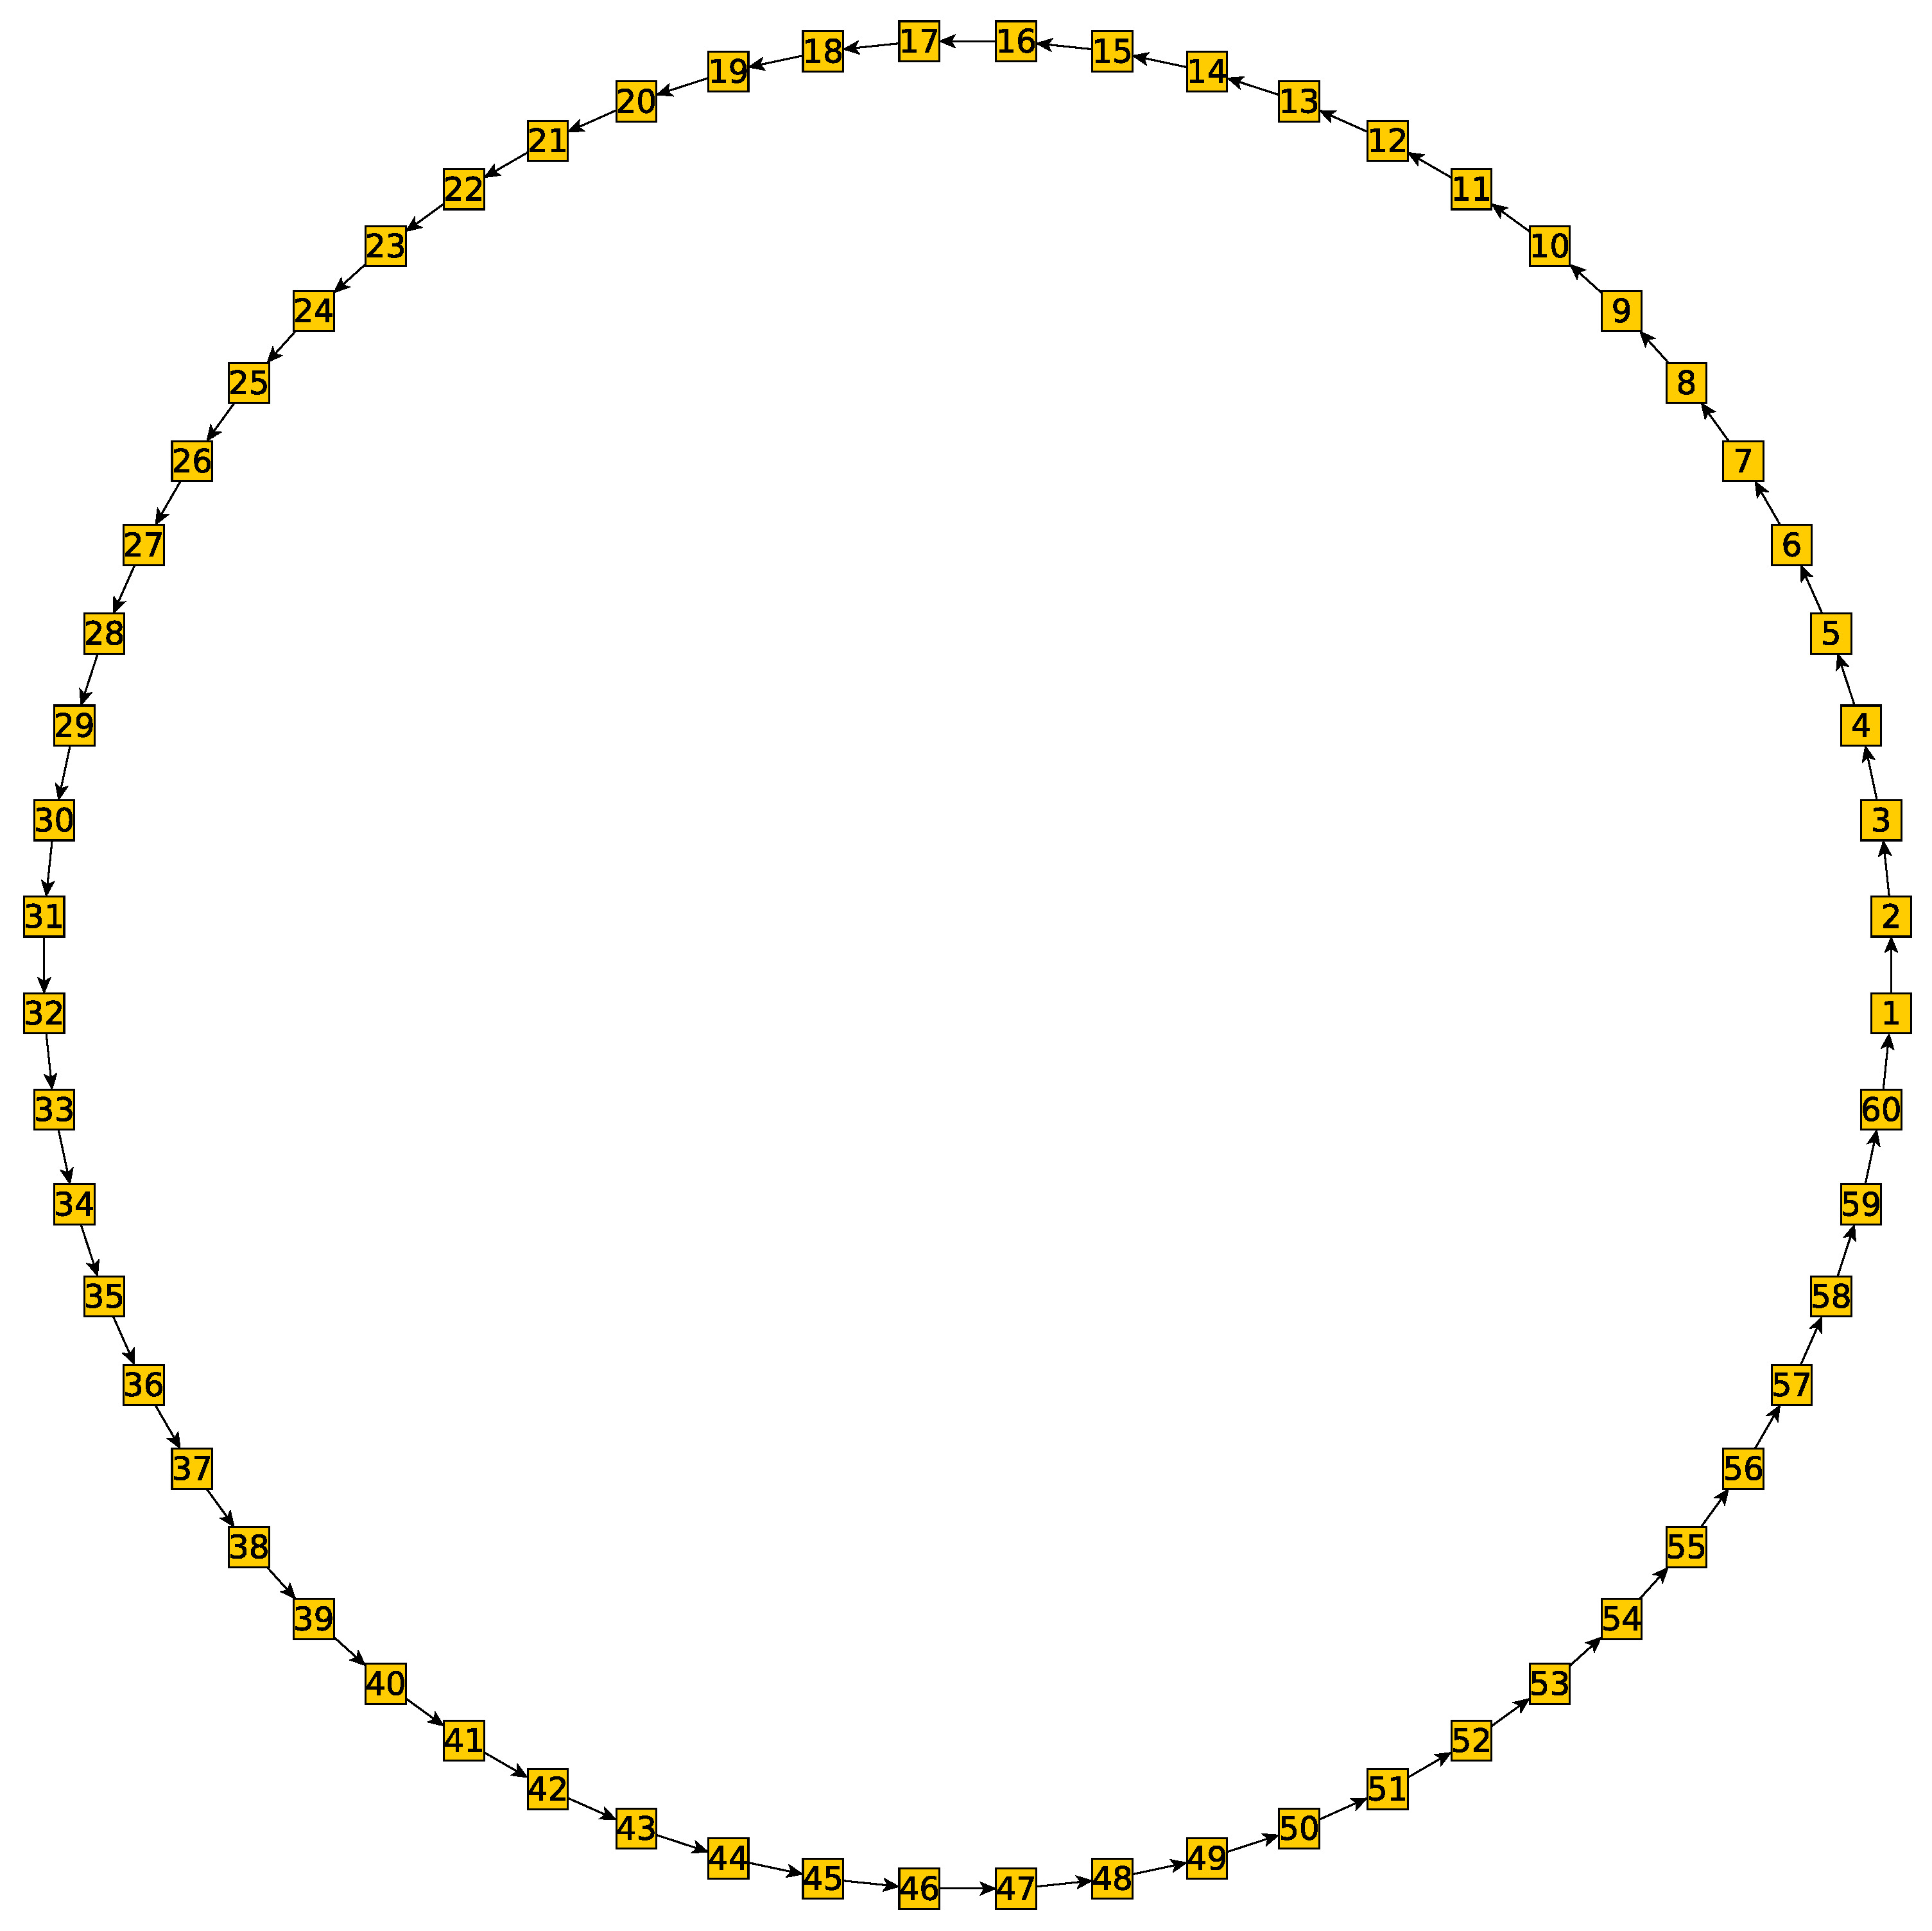
\includegraphics[width=\textwidth]{figures/CircleTests/CircleTestIllustrations/Circle_Test_Graph-No_arc_labels_or_costs.pdf}}
	\caption{Circle Test Graph example with no arc labels or costs drawn in}
	\label{fig:ctgnaloc}
\end{figure}

\begin{figure}[thbp]
	\noindent
	\fbox{
		\parbox{\textwidth}{
			{A1, A2, A3, A4, A5, A6, A7, A8, A9, A10, A11, A12, A13, A14, A15, A16, A17, A18, A19, A20, A21, A22, A23, A24, A25, A26, A27, A28, A29, A30, A31, A32, A33, A34, A35, A36, A37, A38, A39, A40, A41, A42, A43, A44, A45, A46, A47, A48, A49, A50, A51, A52, A53, A54, A55, A56, A57, A58, A59, A60}
		}
	}
	\caption{Best possible genome for the supplied Circle Test example}
	\label{fig:bpgftscte}
\end{figure}

While using the (TODO: referer circle\_test.dat her) might not give an exact answer to what configuration of the parameters is optimal, it still gives a usable prediction of what configurations work in a general case with our implementation. Another limitation that is not adressed at this point is that it only makes sense to evaluate it as giant round trip completed by one vehicle. It could be adopted to facilitate testing splitting the graph between several vehicles by adding a depot node in the center and making edges that are not required to service from it to all the nodes (as illustrated in figure \ref{fig:ctgcdnaoeloc}). However that would add a lot of complexity, and we did not have time to investigate it further.

\begin{figure}[thbp]
	\centerline{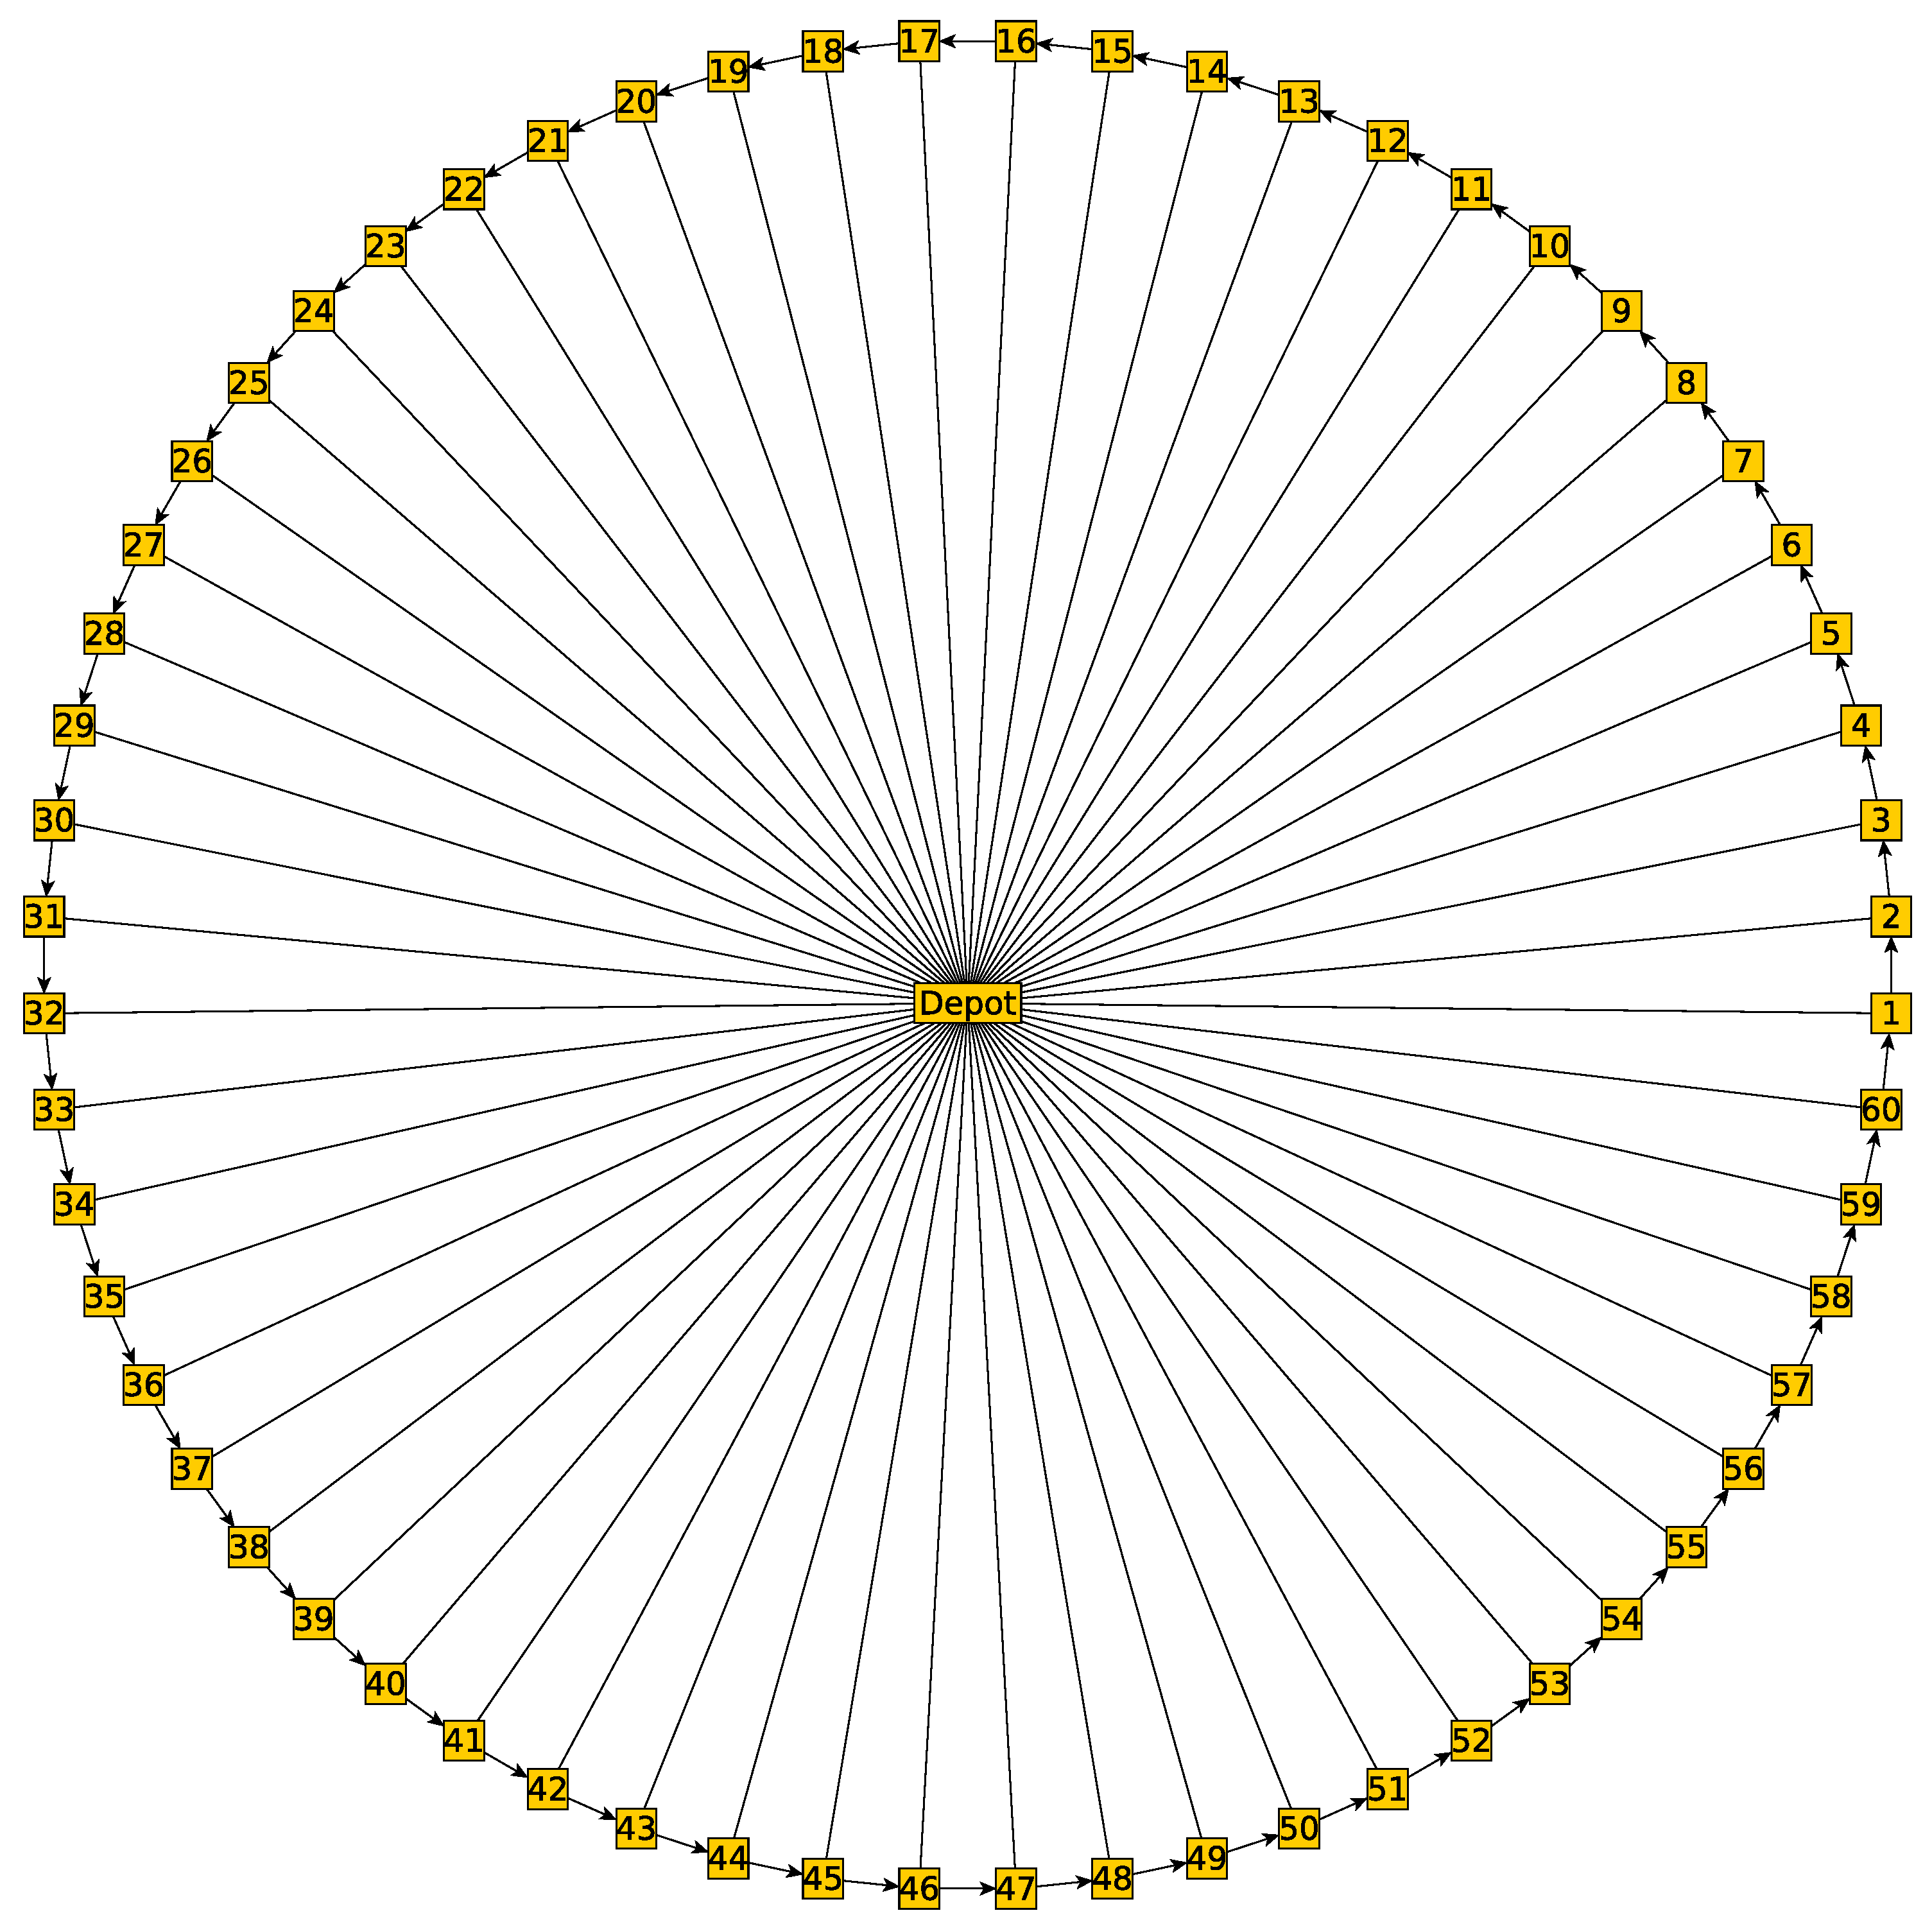
\includegraphics[width=\textwidth]{figures/CircleTests/CircleTestIllustrations/Circle_Test_Graph_Central_Depot-No_arc_or_edge_labels_or_costs.pdf}}
	\caption{Alternative Circle Test Graph example with depot node and no arc labels or costs drawn in}
	\label{fig:ctgcdnaoeloc}
\end{figure}

%Comment on memeticism here?

% section experimental_plan (end)

\section{Experimental Setup} % (fold)
\label{sec:experimental_setup}
% This section should be about how we did the experiments, ie. what parameters we used and so forth
We decided to split the tuning of the EA into three parts. Determining the population size, parent selection, and adult selection. For each part, we would select what parameters we wanted to try. Then we would run each configuration 30 times to gather data about the best results found under the configuration, and the population averages. To make the results as comparable as possible, we chose to let each configuration run for exactly 100000 generations. For each run all the genotypes were initialized randomly, and each 16th generation the best fitness of the population, the average fitness of the population, and the standard deviation of the fitness of the population at that point was recorded.

For determining the population size, we decided that we wanted to try population sizes corresponding to 10\%, 50\%, 100\%, and 200\% of the genome length. When testing it we used uniform selection for parent selection, and full generational replacement for the adult selection.

When testing the parent selection we set the size of the population at 200\% of the genome length, and used full generational replacement for the adult selection, as that allowed us to reuse the results from the population size run for uniform selection.

When trying to find the best way to do the adult selection we used a population size of 200\% of the genome length, and fitness proportionate selection as the parent selection. When testing overproduction we decided to make as many pairs as there are individuals in the population, ie. producing twice as many children as there can be survivors to next generation.
% section experimental_setup (end)

\clearpage

\section{Results} % (fold)
\label{sec:results}

\subsection{Population Size} % (fold)
\label{sub:population_size}

When we observed the results from the population size test runs, we notice that that a lower population size yields better results. The larger populations perform noticeably worse, with the largest population (120 individuals) giving the worst results. This seemed very counterintuitive, especially that a miniscule population of 6 individuals manages to get results that are somewhat good. Therefore we decided to run a control experiment where we used other parent selection and adult selection methods to check if it was the combination of uniform selection and full generational mixing that gave the veird results.

\begin{figure}[thbp]
	\centerline{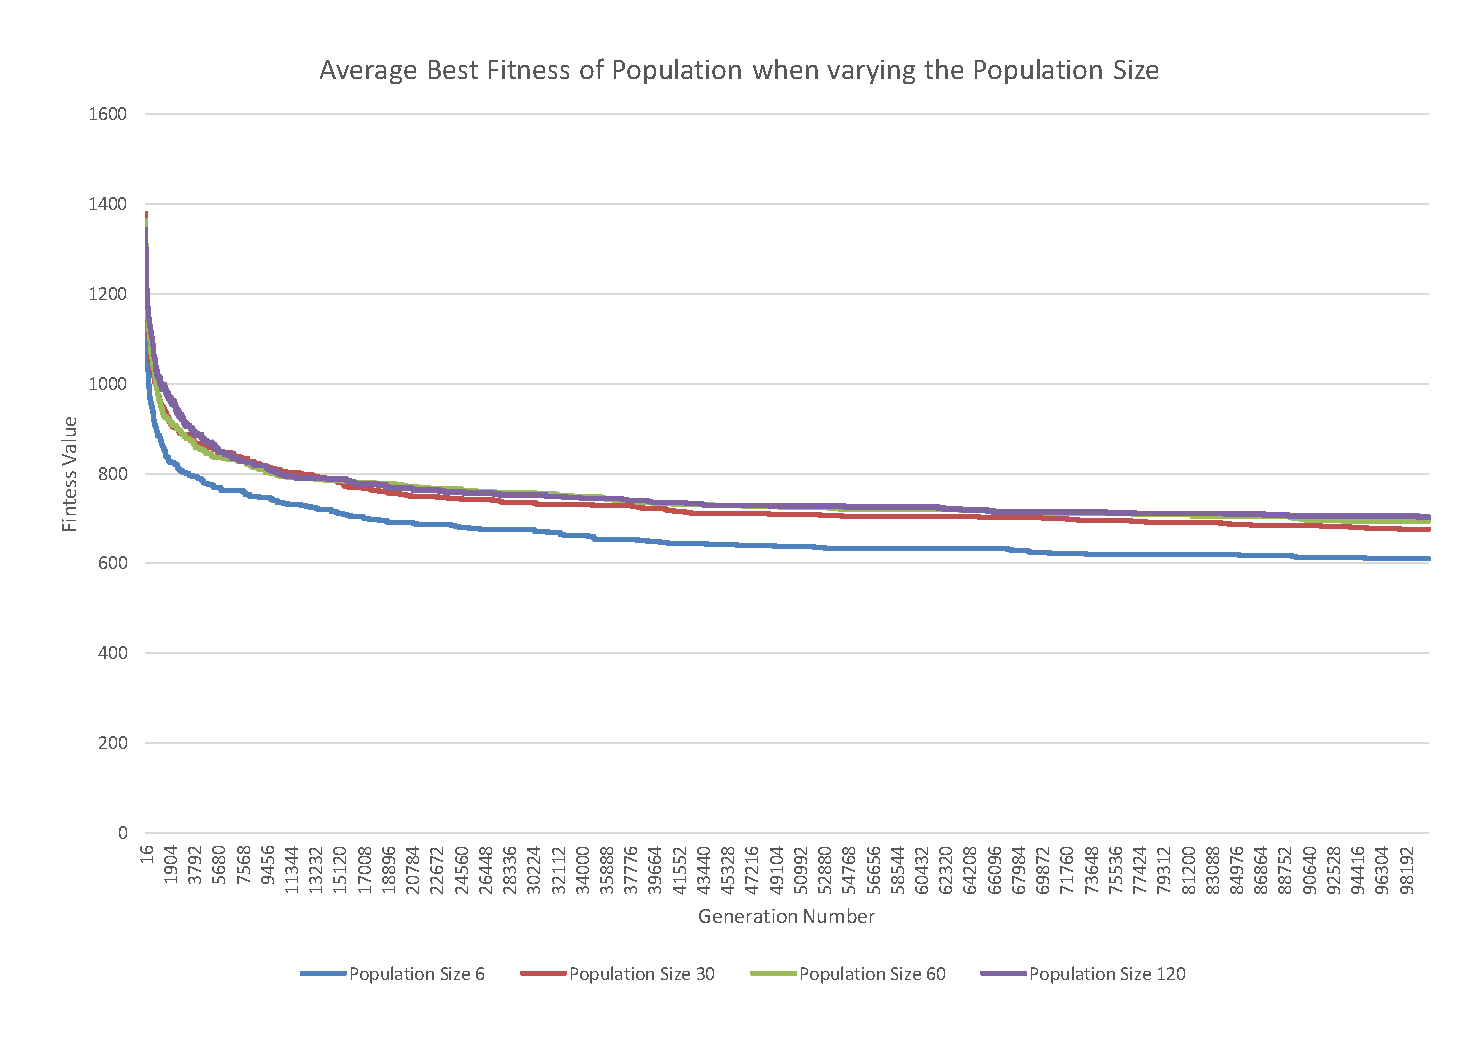
\includegraphics[width=\paperwidth]{figures/CircleTests/CircleTestsPopulationAverageBest.pdf}}
	\caption{Population Size - Average Best}
\end{figure}

\begin{figure}[thbp]
	\centerline{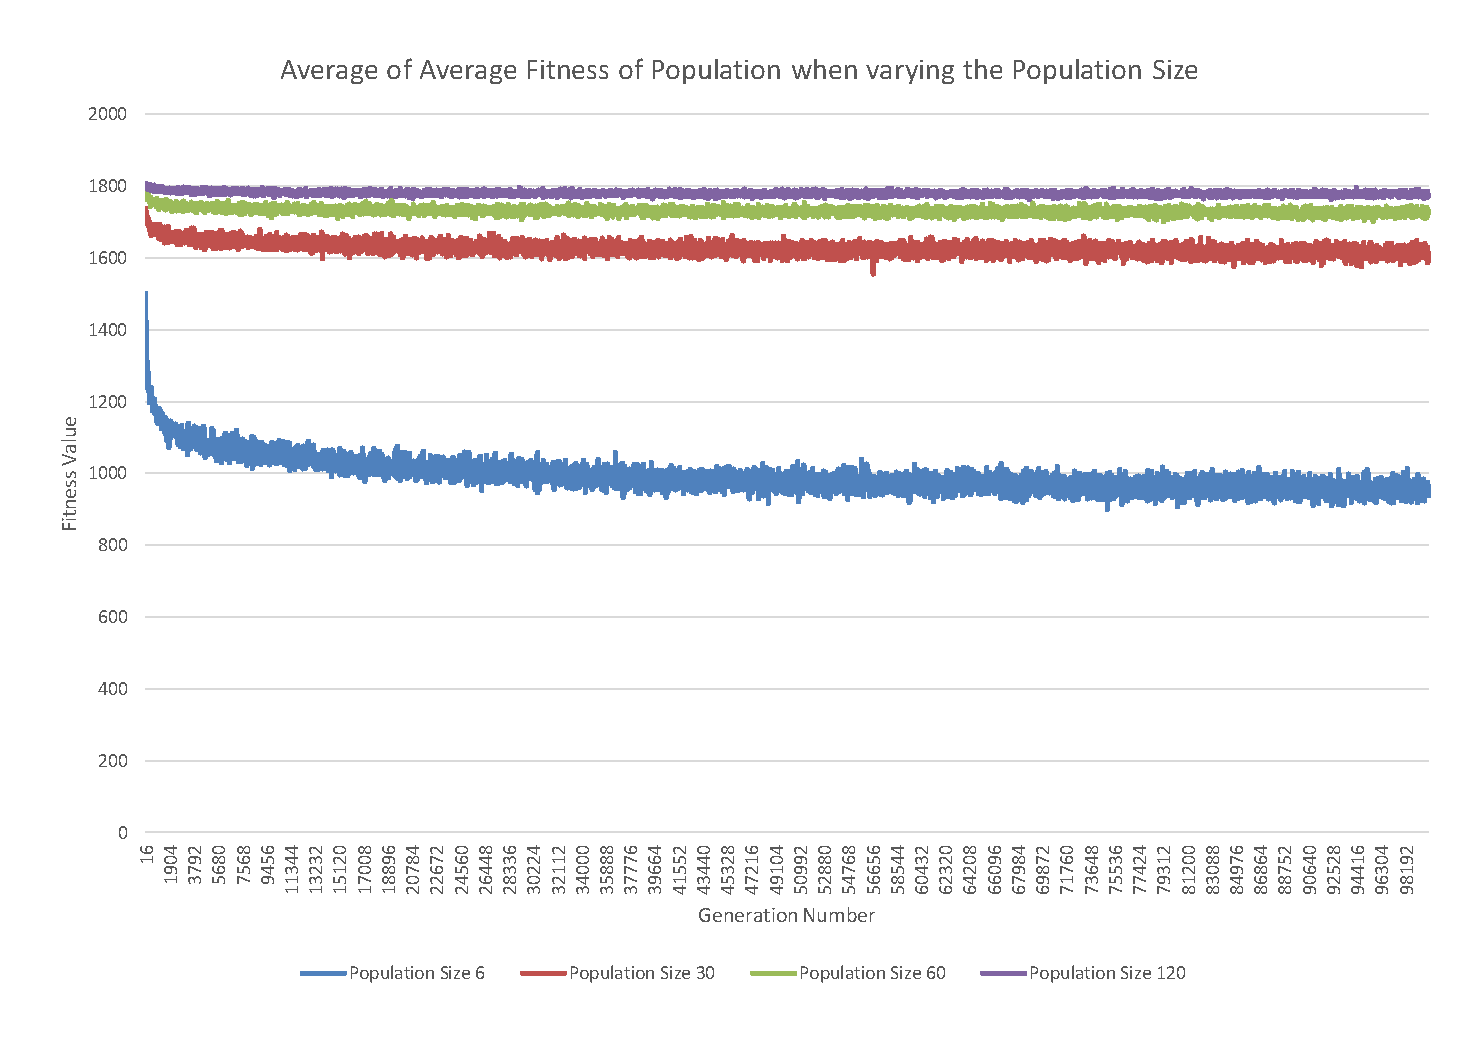
\includegraphics[width=\paperwidth]{figures/CircleTests/CircleTestsPopulationAverageAverage.pdf}}
	\caption{Population Size - Average Average}
\end{figure}

\begin{figure}[thbp]
	\centerline{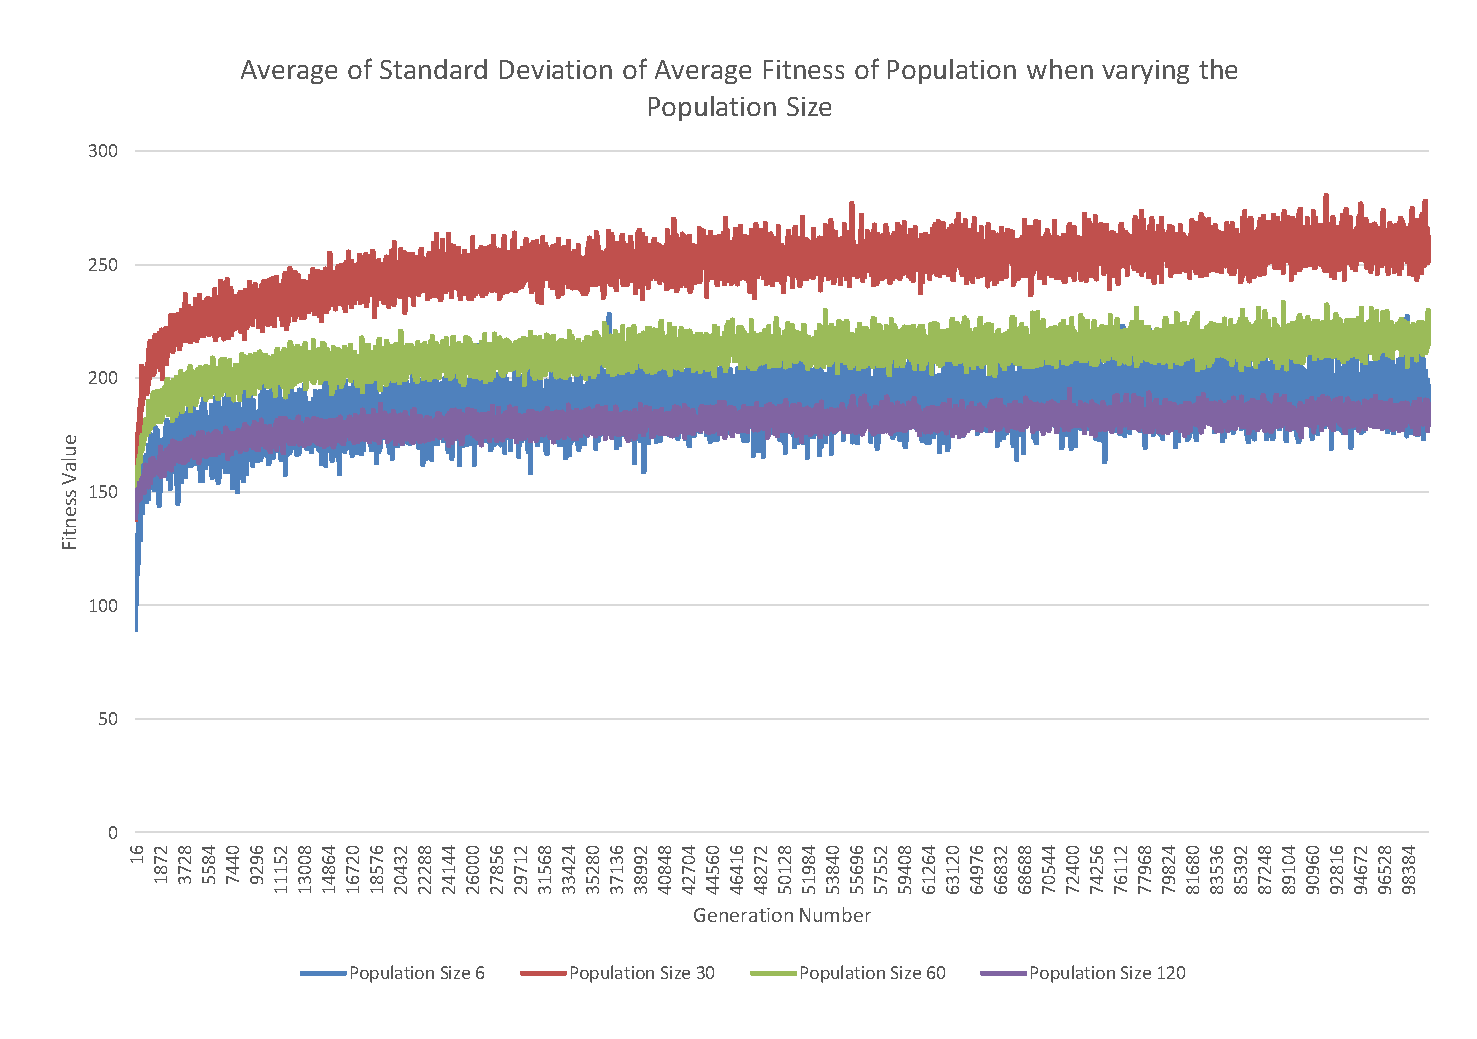
\includegraphics[width=\paperwidth]{figures/CircleTests/CircleTestsPopulationAverageStandardDeviation.pdf}}
	\caption{Population Size - Average Standard Deviation}
\end{figure}
% subsection Population Size (end)

\clearpage

\subsection{Parent Selection} % (fold)
\label{sub:parent_selection}

Here we can see that fitness proportionate selection is clearly better than the tournament selection, which in turn finds better results on average than uniform selection. The averages fitness of each populations average seem to quickly decrease before beginning to decrease slowly for tournament and fitness proportionate selection, while the uniform selection shows only a very slow improvement over time.

\begin{figure}[thbp]
	\centerline{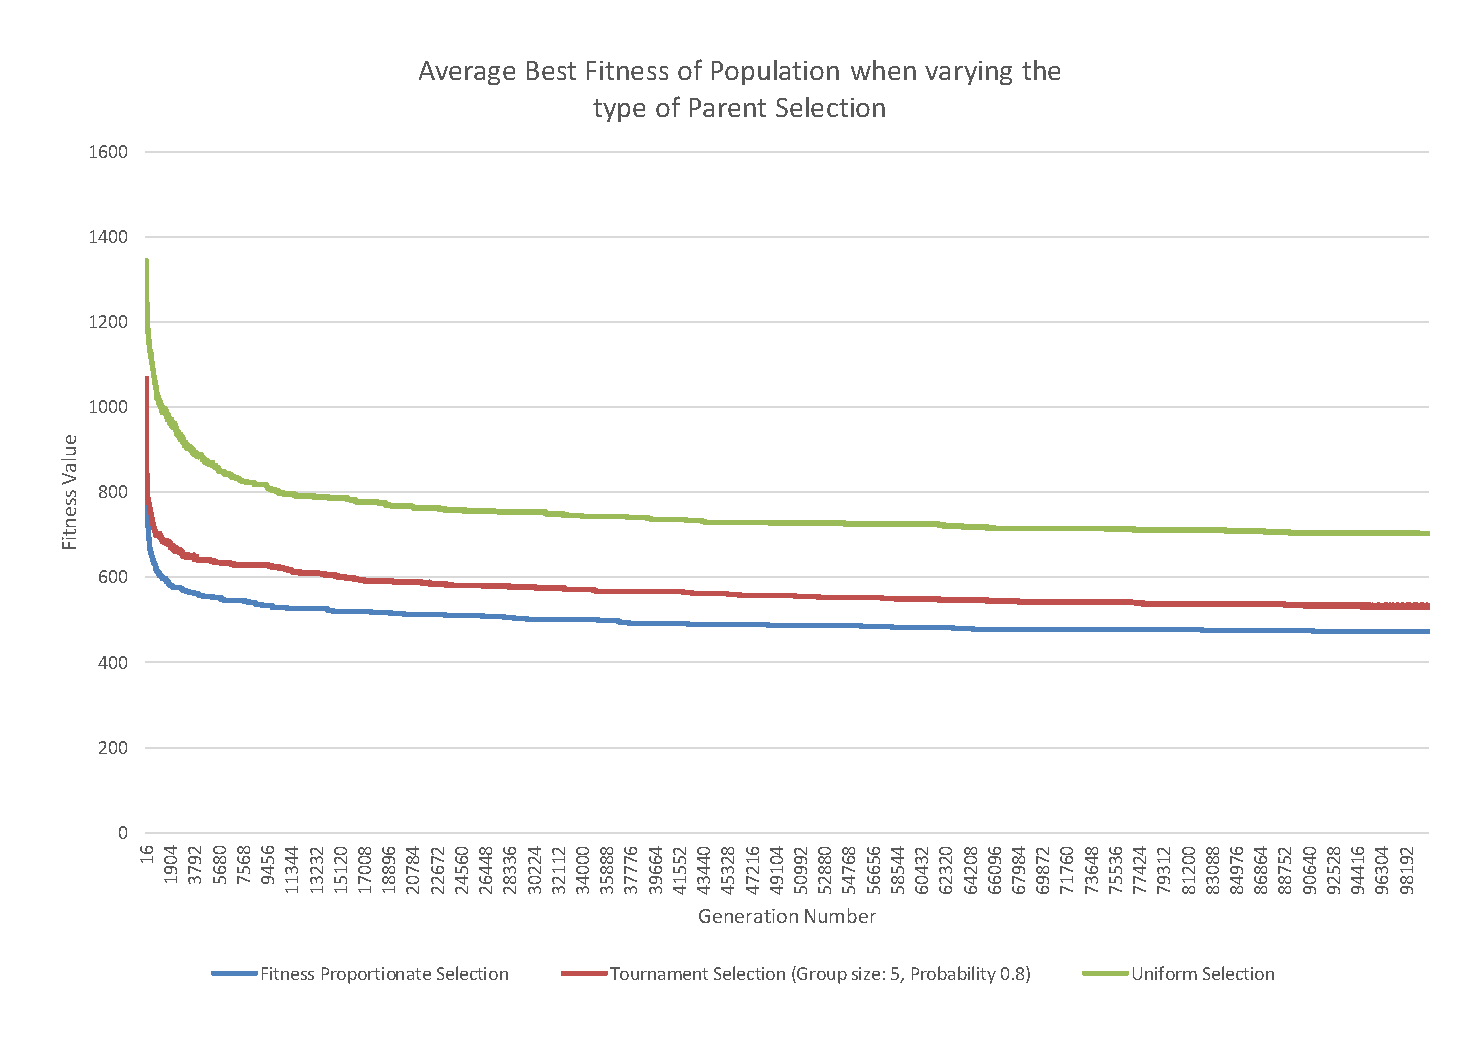
\includegraphics[width=\paperwidth]{figures/CircleTests/CircleTestParentSelectionAverageBest.pdf}}
	\caption{Parent Selection - Average Best}
\end{figure}

\begin{figure}[thbp]
	\centerline{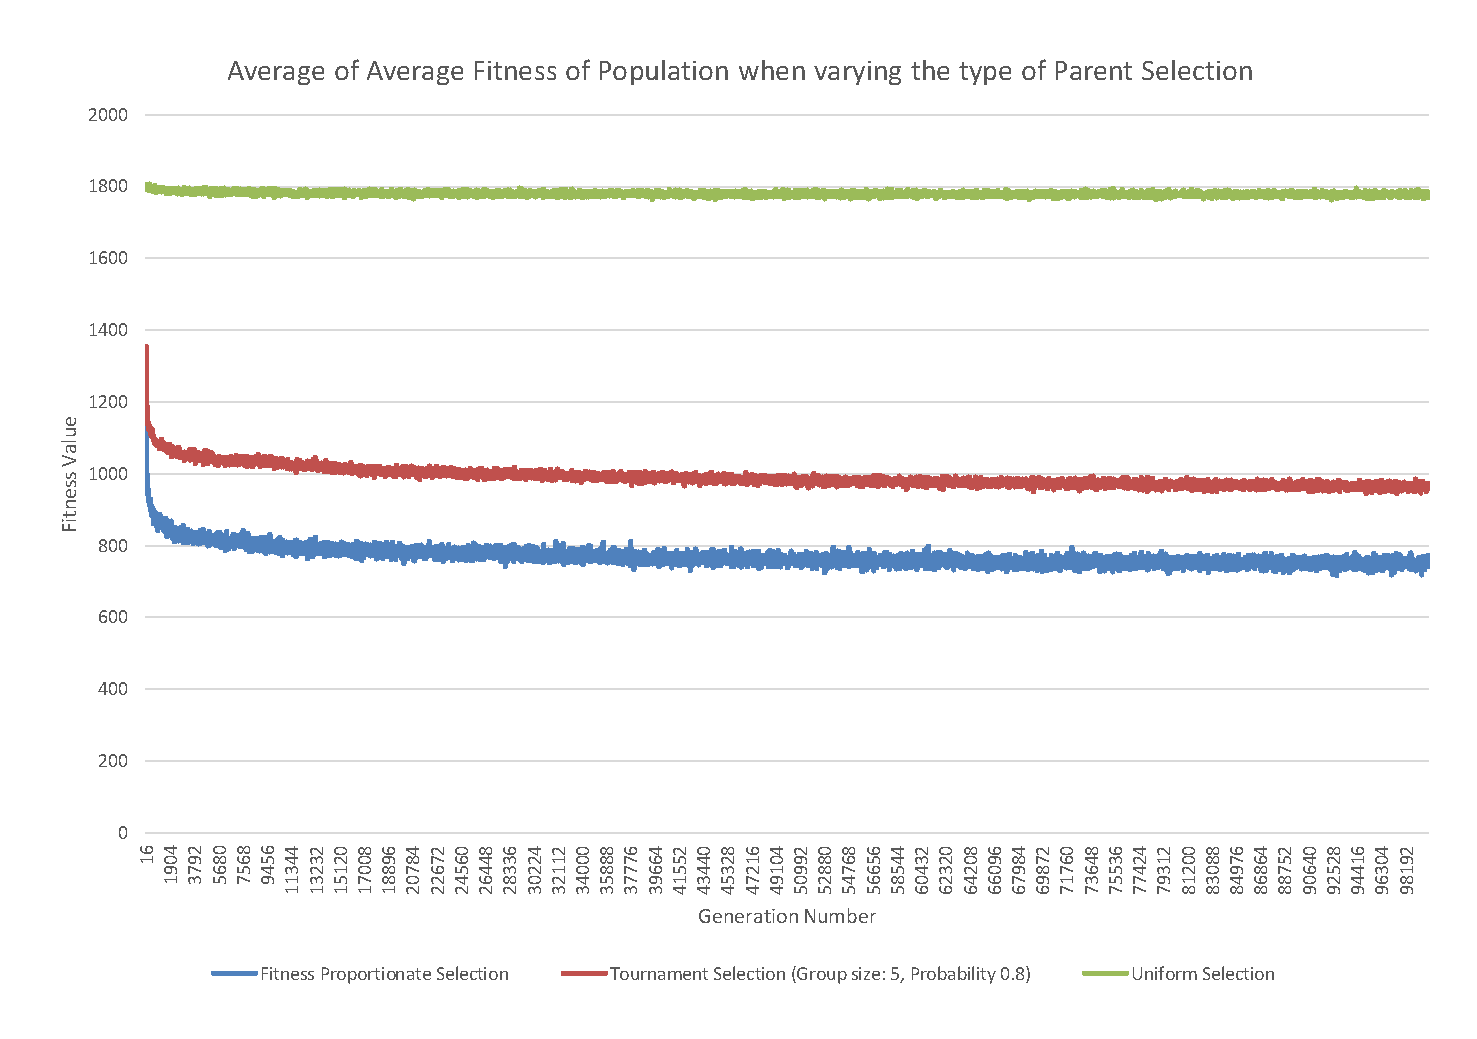
\includegraphics[width=\paperwidth]{figures/CircleTests/CircleTestParentSelectionAverageAverage.pdf}}
	\caption{Parent Selection - Average Average}
\end{figure}

\begin{figure}[thbp]
	\centerline{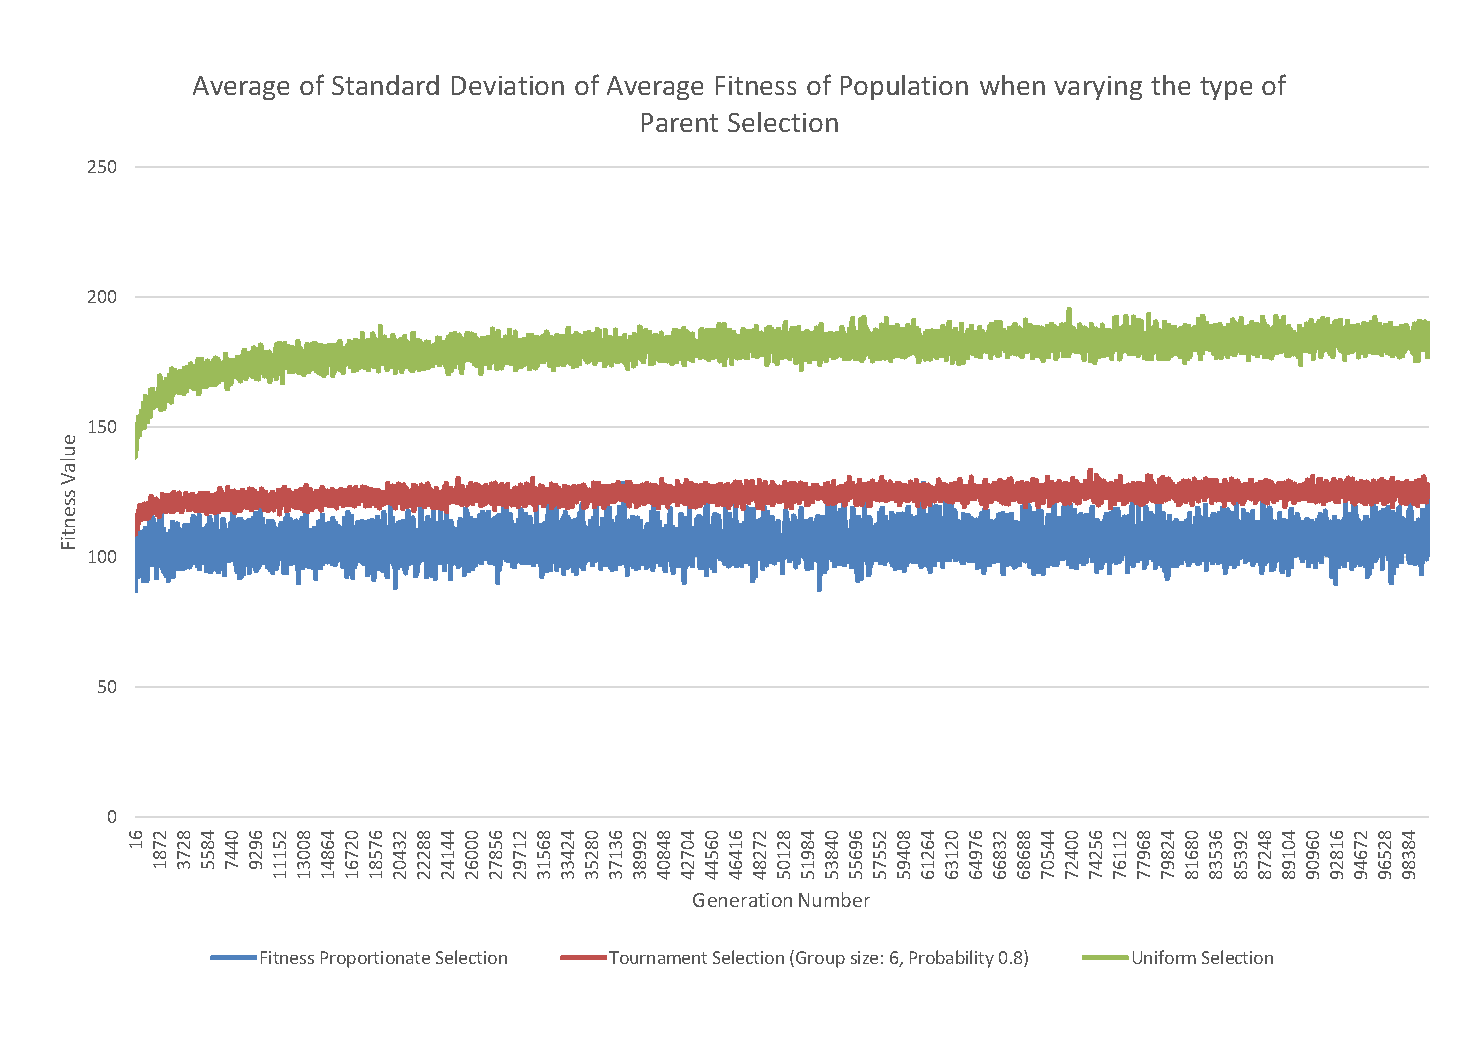
\includegraphics[width=\paperwidth]{figures/CircleTests/CircleTestParentSelectionAverageStandardDeviation.pdf}}
	\caption{Parent Selection - Average Standard Deviation}
\end{figure}
% subsection parent_selection (end)

\clearpage

\subsection{Adult Selection} % (fold)
\label{sub:adult_selection}

When looking at the results for the adult selection, the most striking thing is that completely flat curve for the elitist mixing average best, indicating that there on average is no improvement at all in the best solutions found when using it as adult selection. This can be explained by observing that the average standard deviation in each population is 0 (figure \ref{fig:ctasasd}), indicating that the individuals in the population have the same fitness. What has likely happened is that the population has become stuck in a local optimum, and all the individuals it produces are exact copies of the currently best found solution.

When looking for what parent selection gives the best output according to these results both overproduction and random mixing give better results than elitist mixing, and overproduction yields slightly better results than random mixing.

\begin{figure}[thbp]
	\centerline{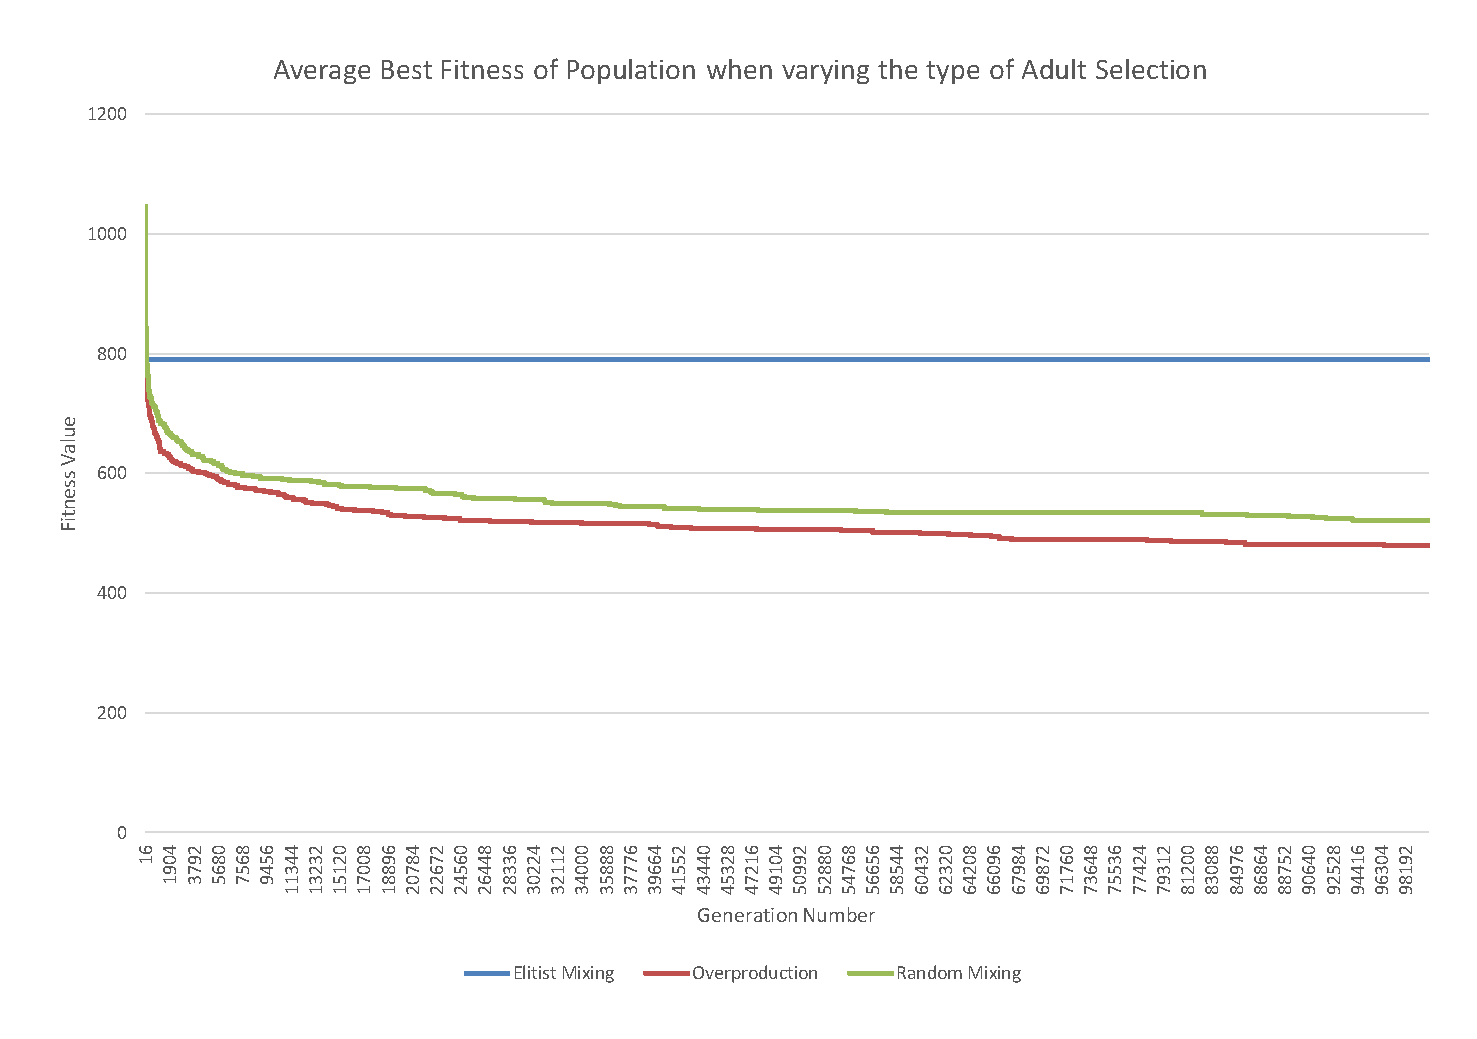
\includegraphics[width=\paperwidth]{figures/CircleTests/CircleTestAdultSelectionAverageBest.pdf}}
	\caption{Adult Selection - Average Best}
\end{figure}

\begin{figure}[thbp]
	\centerline{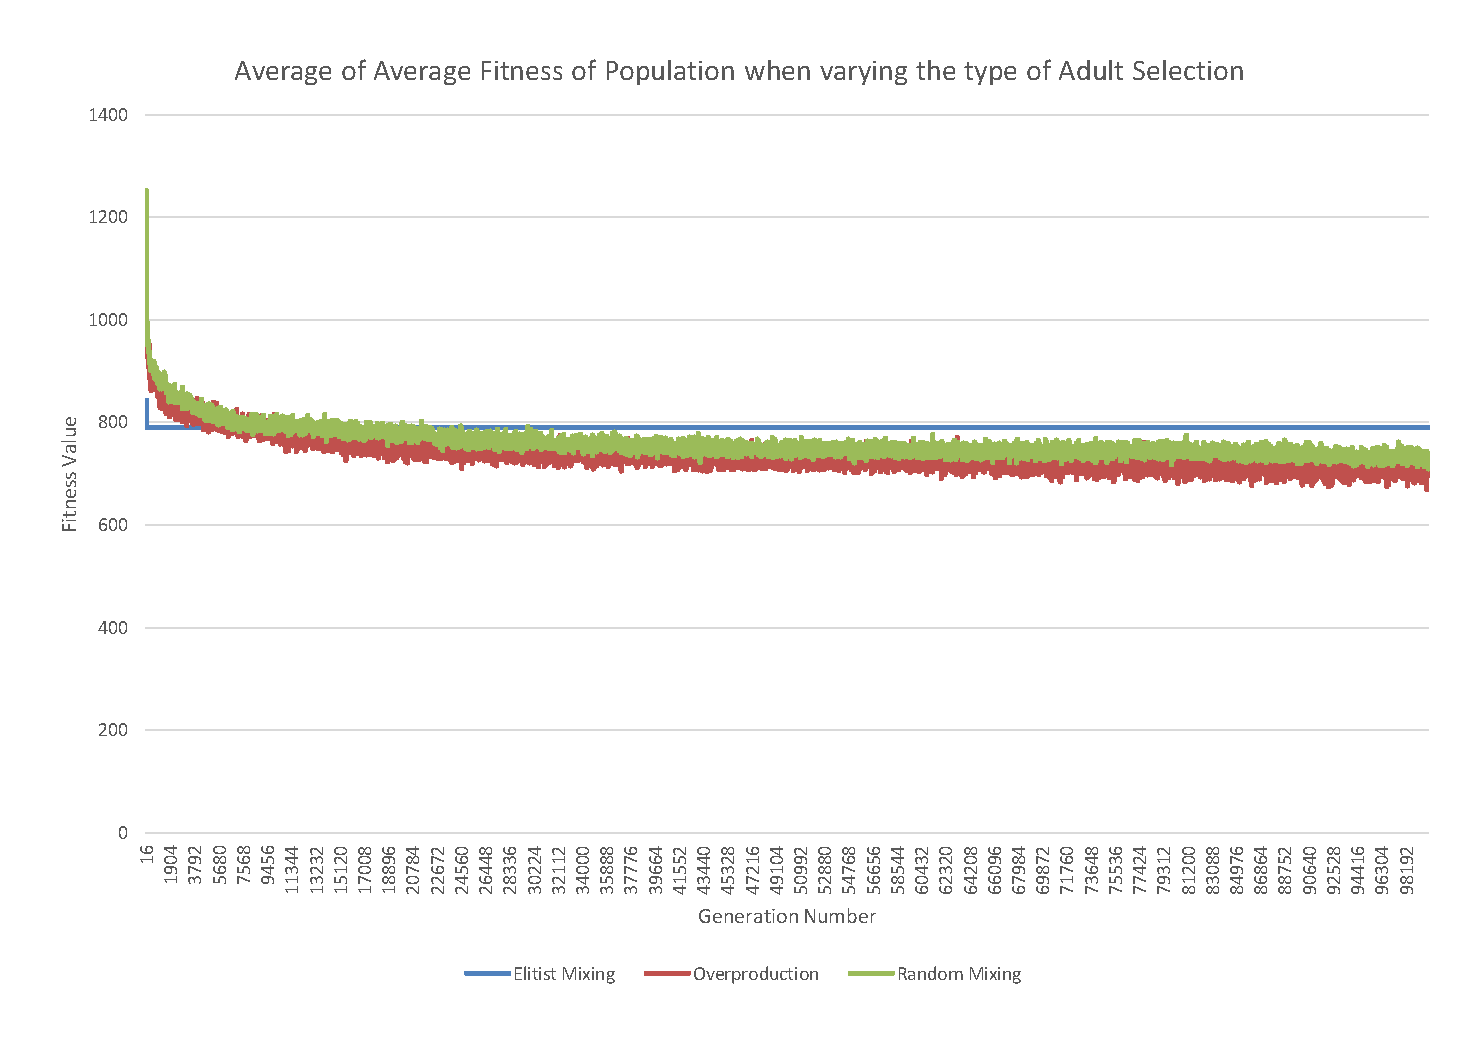
\includegraphics[width=\paperwidth]{figures/CircleTests/CircleTestAdultSelectionAverageAverage.pdf}}
	\caption{Adult Selection - Average Average}
\end{figure}

\begin{figure}[thbp]
	\centerline{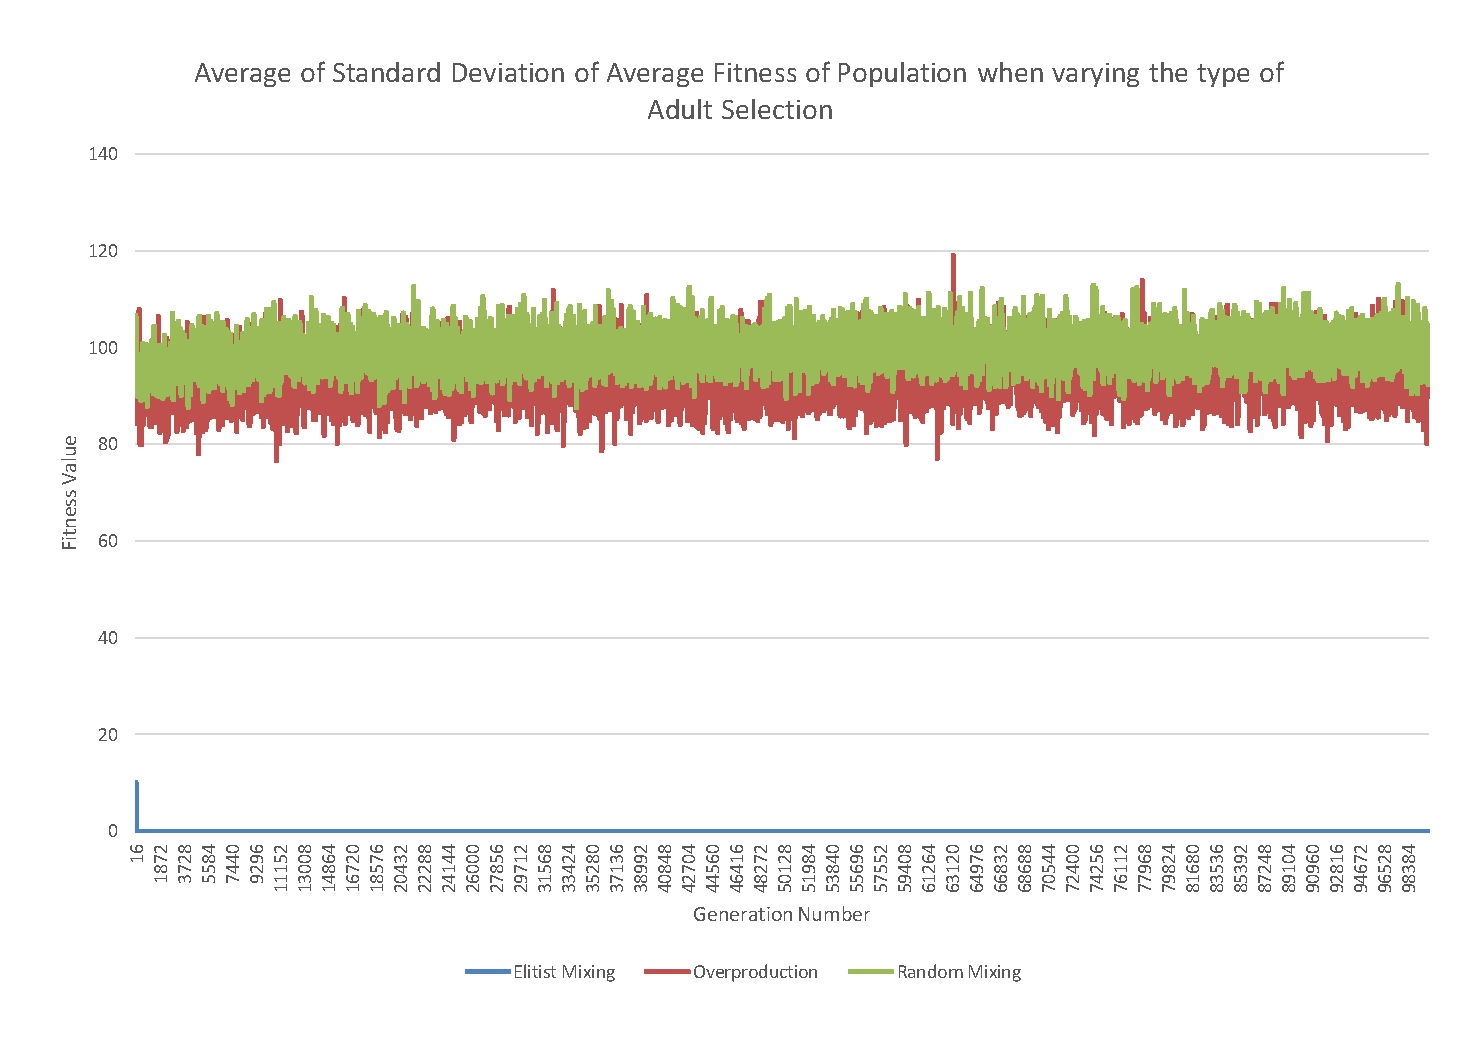
\includegraphics[width=\paperwidth]{figures/CircleTests/CircleTestAdultSelectionAverageStandardDeviation.pdf}}
	\caption{Adult Selection - Average Standard Deviation}
	\label{fig:ctasasd}
\end{figure}
% subsection adult_selection (end)

\clearpage

\subsection{Population Size Control} % (fold)
\label{sub:population_size_control}

Due to the veird in the population size tests (section \ref{sub:population_size}), we decided to look into whether the effect of the population size could be impacted by the choice of uniform parent selection and full generational replacement. We designed a control test where we again ran each population size 30 times, but this time we ran useing fintess scaling selection and overproduction with twice as many children as the population size.

The results we got now were much more in tune with what we had anticipated in the first place. A larger population gives better results, but as the populations grow very large there are diminishing returns on expanding it furgher. As can be seen in figure \ref{fig:cpscab} the largest population gives only marginally better results than the second largest population, which gives somewhat better results than the third largest population, which in turn gives a lot better results than the smallest population.

\begin{figure}[thbp]
	\centerline{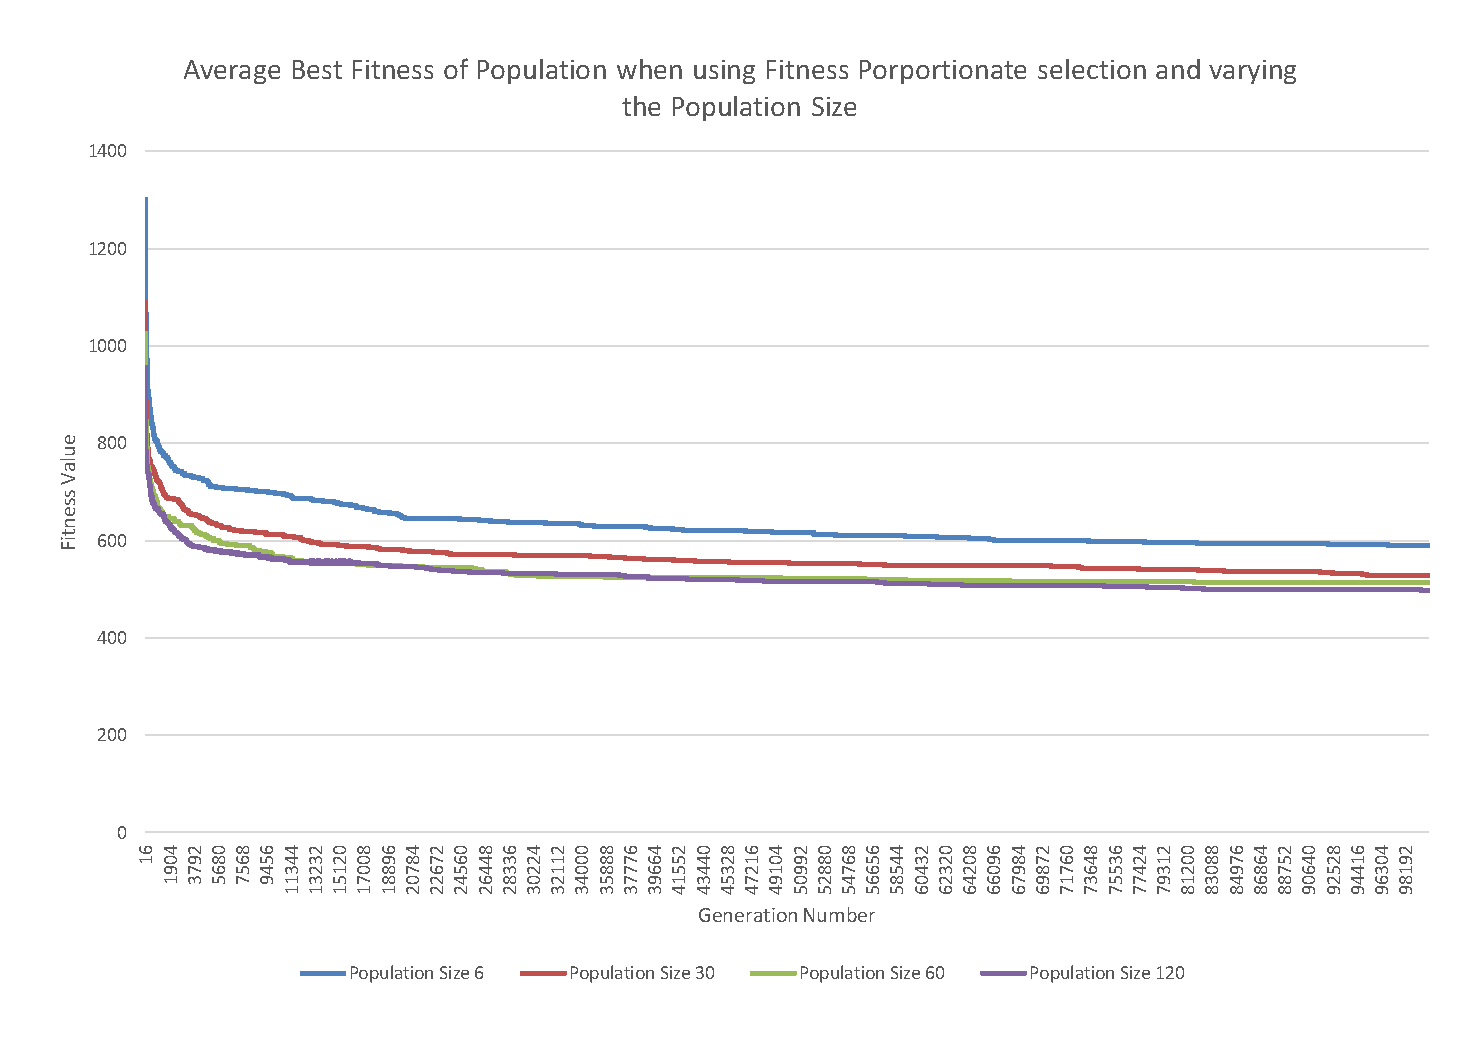
\includegraphics[width=\paperwidth]{figures/CircleTests/CirclePopulationSizeControllAverageBest.pdf}}
	\caption{Population Size Control - Average Best}
	\label{fig:cpscab}
\end{figure}

\begin{figure}[thbp]
	\centerline{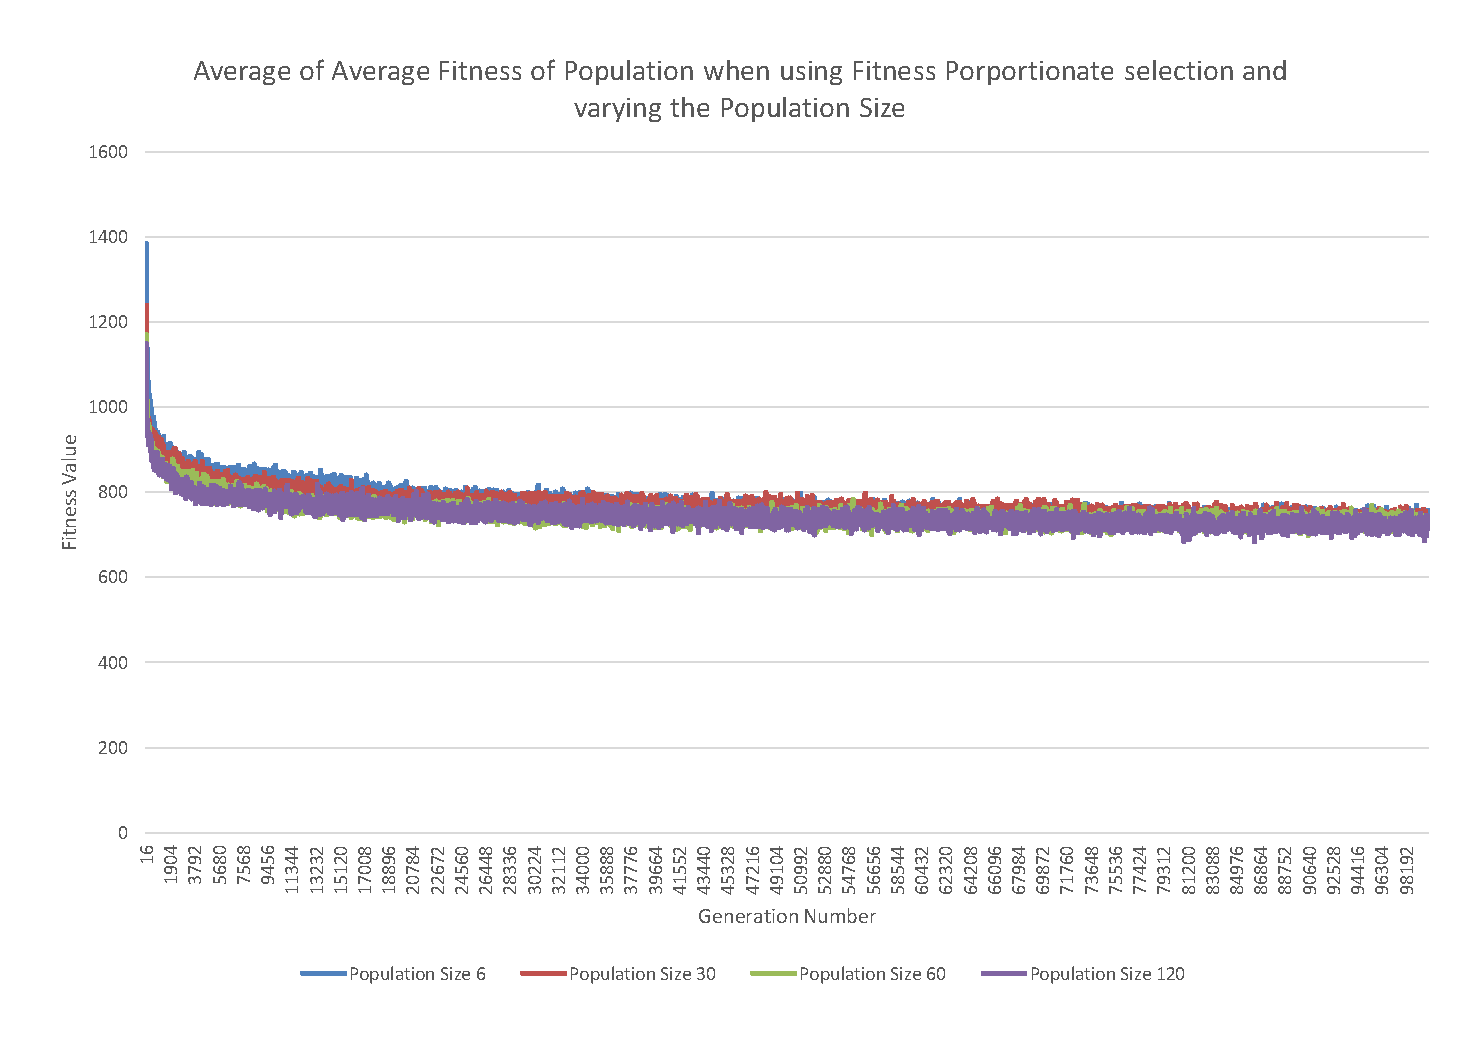
\includegraphics[width=\paperwidth]{figures/CircleTests/CirclePopulationSizeControllAverageAverage.pdf}}
	\caption{Population Size Control - Average Average}
\end{figure}

\begin{figure}[thbp]
	\centerline{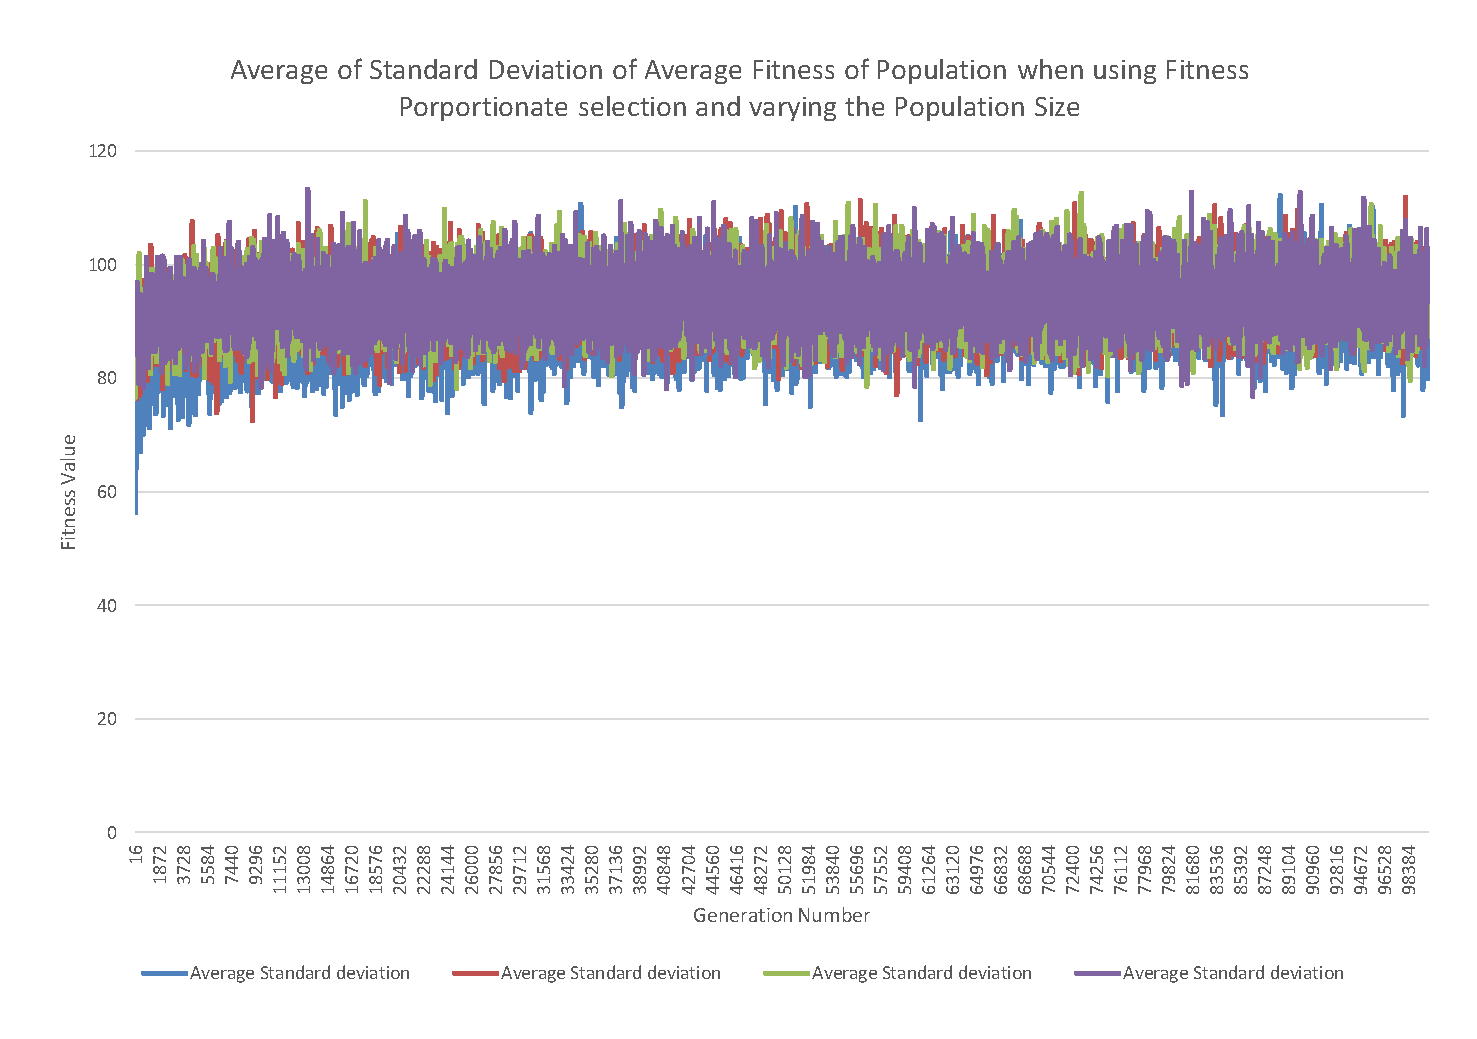
\includegraphics[width=\paperwidth]{figures/CircleTests/CirclePopulationSizeControllAverageStandardDeviation.pdf}}
	\caption{Population Size Control - Average Standard Deviation}
\end{figure}
% subsection population_size_control (end)

\clearpage

% section results (end)

\section{Evaluation and Conclusion} % (fold)
\label{sec:evaluation_and_conclusion}

The above experiments lead us to the following conclusions about the parameters for the EA. Section \ref{sub:parent_selection} indicated that the best parent selection method for our algorithm is fitness proportionate selection. As for the adult selection section \ref{sub:adult_selection} shows that overproduction is the adult selection type that gives the best fitnesses in our implementation. In section \ref{sub:population_size_control} we find that a larger population is better, but it has diminishing returns and a population size of 200\% the length of the genome is not much better than a population size equivalent to 100\% the length of the genome. It contradicts our findings from section \ref{sub:population_size}, but because almost all other configurations yield better results than uniform parent selection combined with full generational replacement as adult selection on its best we choose to regard that as a quirk of the combination.

What could be improved: A test that also tests splitting would be better. Using real world test data would give inidcations as to running time, which would make it better in itself. Furthermore it could give more parameters. Another signifficant limitation is that we did not get time to look into other configurations of the torunament selection. It would be interesting to look into how memetic vs random mutation works on this kind of graph. Also it would be interesting to know why uniform selection coupeled with full generational replacement worked at all given that it essentialy is search by random sort.

% section evaluation_and_conclusion (end)
\cleardoublepage
% chapter evolutionary_algorithm_configuration (end)